\documentclass[varwidth=true, border=2pt]{standalone}
\usepackage{tikz}
\usetikzlibrary{arrows,positioning} 
\tikzset{
    %Define standard arrow tip
    >=stealth',
    % Define arrow style
    pil/.style={->,thick}
}
\tikzstyle{vertex}=[draw,fill=black,circle,minimum size=10pt,inner sep=0pt]
\begin{document}
  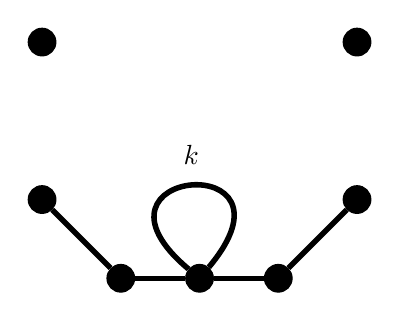
\begin{tikzpicture}
      \node (a)[vertex] at (0,3) {};
      \node (b)[vertex] at (0,1) {};
      \node (c)[vertex] at (1,0) {};
      \node (d)[vertex] at (2,0) {};
      \node (e)[vertex] at (3,0) {};
      \node (f)[vertex] at (4,1) {};
      \node (g)[vertex] at (4,3) {};

      \foreach \from/\to in {b/c,c/d,d/e,e/f}
        \draw[line width=2pt] (\from) -- (\to);

        \path[line width=2pt] (d) edge[ out=140, in=50
                , looseness=0.8, loop
                , distance=2cm]
            node[above=3pt] {$k$} (d);
  \end{tikzpicture}
\end{document}
